% ---------------------------------------------------
% Trabajo Final de Grado
% Author: Fabián González Lence <alu0101549491@ull.edu.es>
% Chapter: Desarrollo
% ----------------------------------------------------

\chapter{Desarrollo} \label{chap:Development}

Cada uno de los cinco proyectos desarrollados recorrió el flujo en cuatro fases descrito en la Sección~\ref{sec:flujo-trabajo} partiendo de los artefactos de diseño referidos en el Capítulo~\ref{chap:Design}. 
Se documenta aquí la ejecución concreta de ese flujo organizado por fases, lo que permite observar la evolución de las herramientas y las incidencias a lo largo de la experiencia. 
El código fuente, los \textit{prompts} y los informes de calidad están disponibles en el repositorio del \ac{TFG} \cite{URL::TFG}.

\section{Fase de Arquitectura} \label{sec:dev-architecture}

En los cinco proyectos, el Arquitecto (Claude) generó en una única interacción la estructura de directorios completa y los esqueletos de clases a partir de la especificación semiformal y los diagramas UML\footnote{Estructuras generadas: \href{https://github.com/alu0101549491/TFG-Fabian-Gonzalez-Lence/blob/main/resources/project-structures/1-TheHangmanGame.md}{\texttt{HANGMAN}}, \href{https://github.com/alu0101549491/TFG-Fabian-Gonzalez-Lence/blob/main/resources/project-structures/2-MusicWebPlayer.md}{\texttt{PLAYER}}, \href{https://github.com/alu0101549491/TFG-Fabian-Gonzalez-Lence/blob/main/resources/project-structures/3-MiniBalatro.md}{\texttt{BALATRO}}, \href{https://github.com/alu0101549491/TFG-Fabian-Gonzalez-Lence/blob/main/resources/project-structures/4-CartographicProjectManager.md}{\texttt{CARTO}}, \href{https://github.com/alu0101549491/TFG-Fabian-Gonzalez-Lence/blob/main/resources/project-structures/5-TennisTournamentManager.md}{\texttt{TENNIS}}}. Los esqueletos reproducían con exactitud las capas arquitectónicas definidas en el Capítulo~\ref{chap:Design} y se integraron en el repositorio sin ajustes en todos los casos. La diferencia entre proyectos fue únicamente de escala: de nueve clases en \ac{HANGMAN} a veinticuatro categorías de codificación en \ac{TENNIS}, con las cuatro capas de \textit{Clean Architecture} replicadas en \textit{frontend} y \textit{backend} para los dos proyectos \textit{fullstack}. A partir de \ac{PLAYER}, Claude incorporó de forma autónoma un \textit{script} de inicialización de directorios, eliminando el paso de creación manual presente en \ac{HANGMAN} y a partir de \ac{CARTO} la integración se hacía de forma automática mediante GitHub Copilot.

\section{Fase de Codificación} \label{sec:dev-coding}

\subsection{P1--P3: codificación modular con Mistral}

En \ac{HANGMAN}, Mistral codificó cada módulo de forma independiente\footnote{\href{https://github.com/alu0101549491/TFG-Fabian-Gonzalez-Lence/tree/main/resources/prompts/1-TheHangmanGame/3-CodigoPorModulo}{\textit{Prompts} de código de \texttt{HANGMAN}}}. La incidencia más destacable surgió en la clase \textit{WordDictionary}: en lugar de externalizar el vocabulario, el modelo lo embebió como un \textit{array} literal dentro del método \textit{initializeAnimalWords()}\footnote{\href{https://github.com/alu0101549491/TFG-Fabian-Gonzalez-Lence/blob/6ade2d937c5fc8507893551a8f82d8d46e6fcbb2/projects/1-TheHangmanGame/src/models/word-dictionary.ts\#L46-L54}{\texttt{word-dictionary.ts} — versión inicial con \textit{array} embebido}}, introduciendo deuda de mantenibilidad que se trasladó a la fase de revisión.

En \ac{PLAYER}, la codificación se articuló en dos etapas ---base del \textit{frontend}\footnote{\href{https://github.com/alu0101549491/TFG-Fabian-Gonzalez-Lence/blob/main/resources/prompts/2-MusicWebPlayer/2-CodigoFrontend/frontend.prompt.md}{\textit{Prompt} de \textit{frontend} base}} y codificación modular\footnote{\href{https://github.com/alu0101549491/TFG-Fabian-Gonzalez-Lence/tree/main/resources/prompts/2-MusicWebPlayer/3-CodigoPorModulo}{\textit{Prompts} de código por módulo}}--- y se amplió con tres funcionalidades no priorizadas inicialmente: los modos \textit{Repeat} y \textit{Shuffle} y el control de volumen. Antes de pasar a revisión se corrigieron dos errores: la función \textit{addSong()} del fichero \texttt{usePlaylist.ts}\footnote{\href{https://github.com/alu0101549491/TFG-Fabian-Gonzalez-Lence/blob/main/projects/2-MusicWebPlayer/src/hooks/usePlaylist.ts\#L138-L152}{\texttt{usePlaylist.ts}, líneas 138--152}} no actualizaba el estado correctamente, y el \textit{useEffect()} de autoavance entre canciones en el fichero \texttt{Player.tsx}\footnote{\href{https://github.com/alu0101549491/TFG-Fabian-Gonzalez-Lence/blob/main/projects/2-MusicWebPlayer/src/components/Player.tsx\#L213-L243}{\texttt{Player.tsx}, líneas 213--243}} estaba roto.

En \ac{BALATRO}, la complejidad del dominio determinó una articulación de ficheros distribuidos en grupos funcionales: diez \textit{prompts} cubrieron el núcleo, las manos de póker, el sistema de puntuación, \textit{Blinds}, las cartas especiales, los servicios, los controladores, los componentes React, el gestor de estado y las utilidades\footnote{\href{https://github.com/alu0101549491/TFG-Fabian-Gonzalez-Lence/tree/main/resources/prompts/3-MiniBalatro/3-CodigoPorGrupodeModulos}{\textit{Prompts} de código por grupos}}. 
La ejecución real del juego motivó una fase de corrección previa a la revisión formal con 64 incidencias documentadas\footnote{\href{https://github.com/alu0101549491/TFG-Fabian-Gonzalez-Lence/blob/main/projects/3-MiniBalatro/docs/DEVELOPMENT-LOG-SUMMARIZED.md}{Registro de desarrollo de \texttt{BALATRO}}}. 
Las más representativas se agrupan en cuatro áreas: en la interfaz, la disposición inicial era completamente vertical (véase la Figura~\ref{fig:balatro-ui-before-after}) y se rediseñó en su totalidad, añadiendo los cuatro modales previstos en la especificación que el código no había implementado y generando los recursos gráficos de \textit{jokers}, planetas y \textit{tarots} mediante Google Gemini\footnote{\href{https://gemini.google.com/share/f1833db31105}{Conversación de Gemini con la generación de recursos de \texttt{BALATRO}}}; en la lógica de juego, se corrigió la detección de la escalera baja y se creó la clase \textit{PermanentUpgradeJoker} para un \textit{joker} cuyo efecto no era realizable con la jerarquía generada; en la persistencia, la deserialización de cartas especiales requirió el patrón \textit{Factory} \cite{Chochlik:2016:Factory}, ya que sin él las subclases concretas no podían reconstruirse al recargar la página; y en los \textit{Boss Blinds}, la mecánica de \textit{The Mouth} no había sido implementada y requirió varias iteraciones.

\begin{figure}[H]
  \centering
  \begin{minipage}[b]{0.48\textwidth}
    \centering
    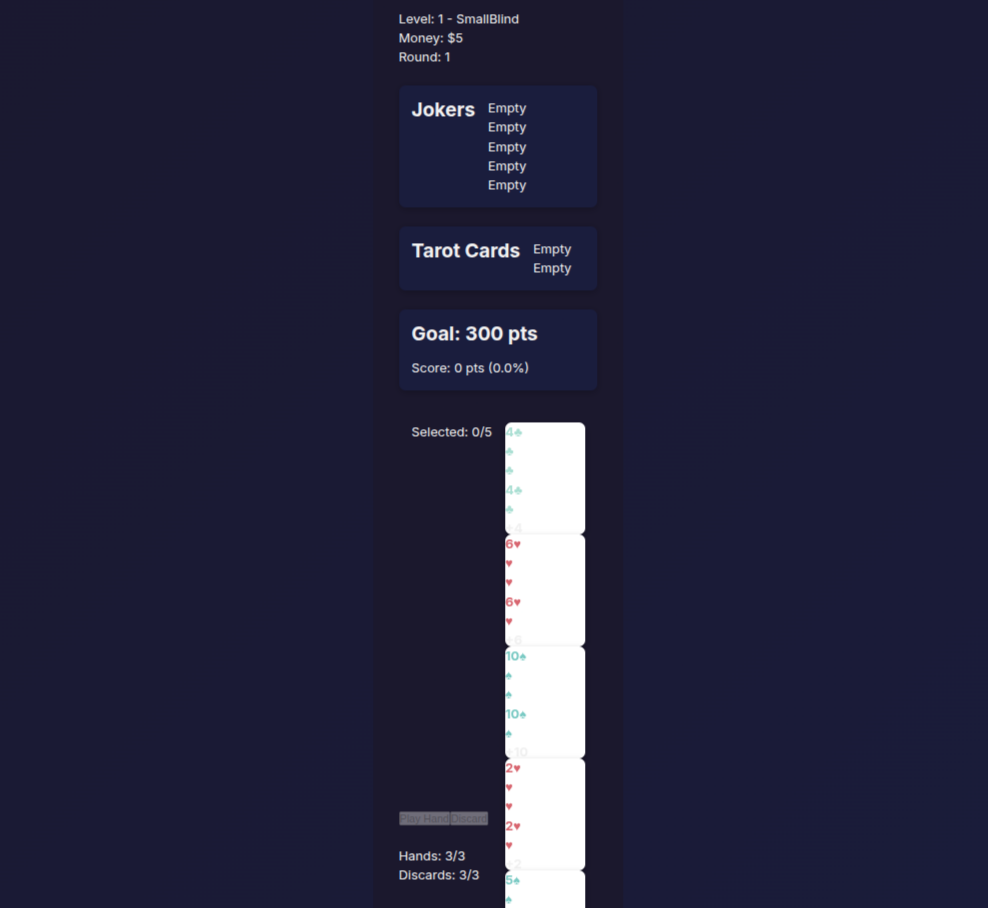
\includegraphics[width=\textwidth]{images/balatro-ui-before}
    %\caption*{\textit{Antes}: disposición vertical generada.}
  \end{minipage}
  \hfill
  \begin{minipage}[b]{0.48\textwidth}
    \centering
    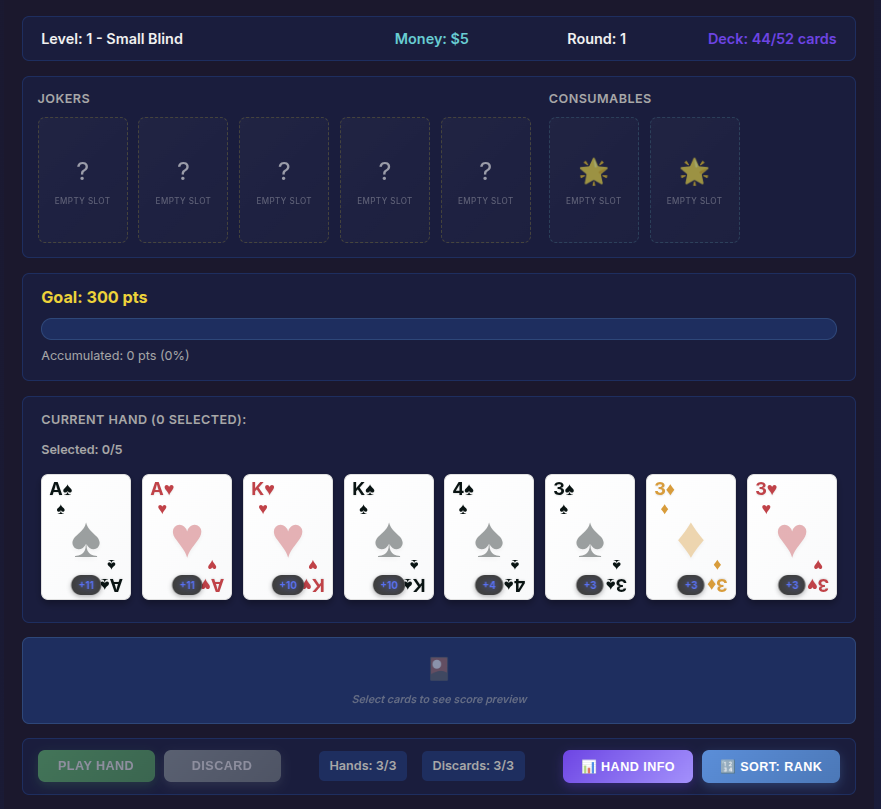
\includegraphics[width=\textwidth]{images/balatro-ui-after}
    %\caption*{\textit{Después}: cambios tras la corrección.}
  \end{minipage}
  \caption{Interfaz de \ac{BALATRO} antes (izquierda) y después (derecha) de la fase de corrección de errores.}
  \label{fig:balatro-ui-before-after}
\end{figure}

\subsection{P4--P5: codificación basada en agentes}

En \ac{CARTO}, el agente cubrió veintiséis grupos de módulos\footnote{\href{https://github.com/alu0101549491/TFG-Fabian-Gonzalez-Lence/tree/main/resources/prompts/4-CartographicProjectManager/3-CodigoPorGruposdeModulos}{\textit{Prompts} de código por grupos}} y operó directamente sobre el sistema de ficheros, resolviendo de forma autónoma los errores de incoherencia intermodular. La fase de integración verificó la comunicación entre todos los módulos y la base de datos: el cliente HTTP se configuró con interceptores Axios para la inyección y renovación silenciosa de \textit{tokens}, que se migraron al \texttt{sessionStorage} del navegador, y los siete módulos de repositorio del \textit{frontend} se alinearon con las rutas del \textit{backend} sin modificaciones de interfaz. El agente implementó también un sistema de notificaciones por WhatsApp mediante la \ac{API} de Twilio\footnote{\href{https://www.twilio.com/en-us/messaging/channels/whatsapp?cq_plac=&cq_net=g&cq_pos=&cq_med=&cq_plt=gp&gad_campaignid=23476018559}{Twilio}} que fue descartado antes de la revisión por no encajar con el alcance del proyecto, eliminando todo el código y los campos del esquema asociados.

En el proyecto \ac{TENNIS}, el agente comenzó definiendo mediante un \textit{prompt} de planificación\footnote{\href{https://github.com/alu0101549491/TFG-Fabian-Gonzalez-Lence/blob/main/resources/prompts/5-TennisTournamentManager/3-Codificacion/planning.prompt.md}{\textit{Prompt} de planificación}} las 24 categorías de codificación y su orden de dependencia\footnote{\href{https://github.com/alu0101549491/TFG-Fabian-Gonzalez-Lence/blob/main/projects/5-TennisTournamentManager/docs/code/CODIFICATION-PROGRESS.md}{\texttt{CODIFICATION-PROGRESS.md} de \texttt{TENNIS}}} e implementó el \textit{frontend} de forma continua\footnote{\href{https://github.com/alu0101549491/TFG-Fabian-Gonzalez-Lence/blob/main/resources/prompts/5-TennisTournamentManager/3-Codificacion/codification.prompt.md}{\textit{Prompt} de codificación}}; el \textit{backend} en Express con: 21 controladores, 14 servicios de aplicación, \textit{middleware} de autenticación, configuración de TypeORM\footnote{\href{https://typeorm.io/}{TypeORM}} y servidor \textit{WebSocket}, se generó en una segunda sesión dedicada\footnote{\href{https://github.com/alu0101549491/TFG-Fabian-Gonzalez-Lence/blob/main/resources/prompts/5-TennisTournamentManager/3-Codificacion/backend.prompt.md}{\textit{Prompt} de \textit{backend}}}. Al probar la aplicación, la interfaz presentaba únicamente una página en blanco. El agente analizó la base de código y generó el fichero \texttt{IMPLEMENTATION\_STATUS.md}\footnote{\href{https://github.com/alu0101549491/TFG-Fabian-Gonzalez-Lence/blob/main/projects/5-TennisTournamentManager/docs/IMPLEMENTATION_STATUS.md}{\texttt{IMPLEMENTATION\_STATUS.md} de \texttt{TENNIS}}}, que cifraba la completitud en torno al 15--20\% e identificaba cinco bloqueadores: la generación de cuadros para los tres formatos de torneo, el algoritmo de cabezas de serie, la resolución de empates en clasificaciones, la gestión de los nueve estados de inscripción y el flujo de confirmación de resultados.

La corrección avanzó durante cuatro semanas. 
En una primera etapa se resolvieron los bloqueadores: los tres generadores de cuadros, el sistema de semillas con colocación estratégica por cuartiles, los seis criterios de desempate encadenados y el ciclo completo de confirmación de resultados con transición a estado en disputa. En una segunda etapa se implementaron las funcionalidades de mayor alcance: el módulo de Orden de Juego con asignación automática de pistas, exportación de estadísticas a cuatro formatos ---PDF, Excel, CSV-ITF y TODS---, el sistema de notificaciones en tiempo real, el tablón de anuncios y los permisos de privacidad de perfiles. La funcionalidad de mayor envergadura fue el soporte para torneos de dobles: la suposición de que un \textit{slot} de cuadro equivalía a un identificador de usuario estaba embebida en aproximadamente 30 ficheros de ambas capas, por lo que se introdujo la entidad \textit{DoublesTeam} y se adaptaron los módulos de cuadros, clasificaciones, estadísticas y visualización. A mitad del proceso, un reescaneo sistemático de la base de código identificó requisitos menores no cubiertos que se completaron antes de cerrar la fase. El proceso evidenció dos patrones de interacción útiles: los errores de integración se resolvían más eficazmente transmitiendo hipótesis concretas al agente sobre su posible causa raíz, ya que desde el propio criterio del desarrollador humano se pudo guiar el comportamiento de la \ac{IA} desarrolladora para depurar secciones concretas de la aplicación; por otro lado, las inconsistencias de estilo se corregían referenciando componentes ya implementados como modelo de referencia en lugar de tener que describir la distribución esperada en texto. 
La Figura~\ref{fig:tennis-ui-before-after} muestra el aspecto de la aplicación al principio y al final de su desarrollo.

\begin{figure}[H]
  \centering
  \begin{minipage}[b]{0.48\textwidth}
    \centering
    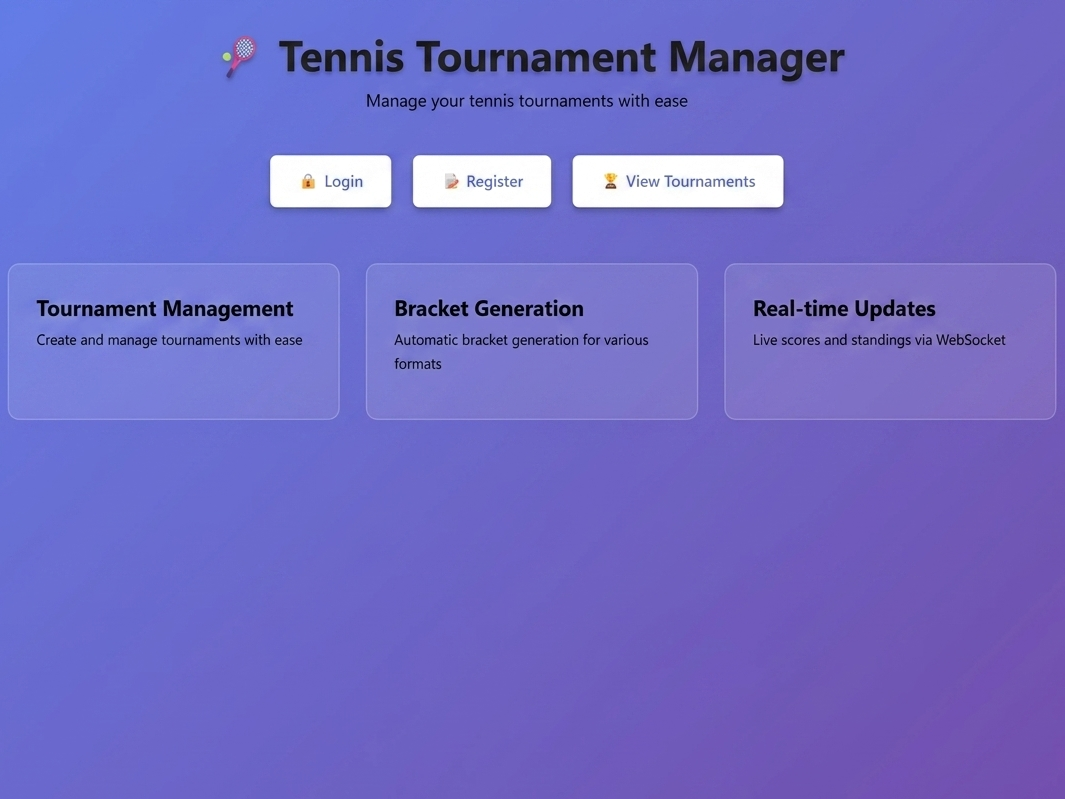
\includegraphics[width=\textwidth]{images/tennis-ui-before}
    %\caption*{\textit{Antes}: diseño inconsistente entre páginas.}
  \end{minipage}
  \hfill
  \begin{minipage}[b]{0.48\textwidth}
    \centering
    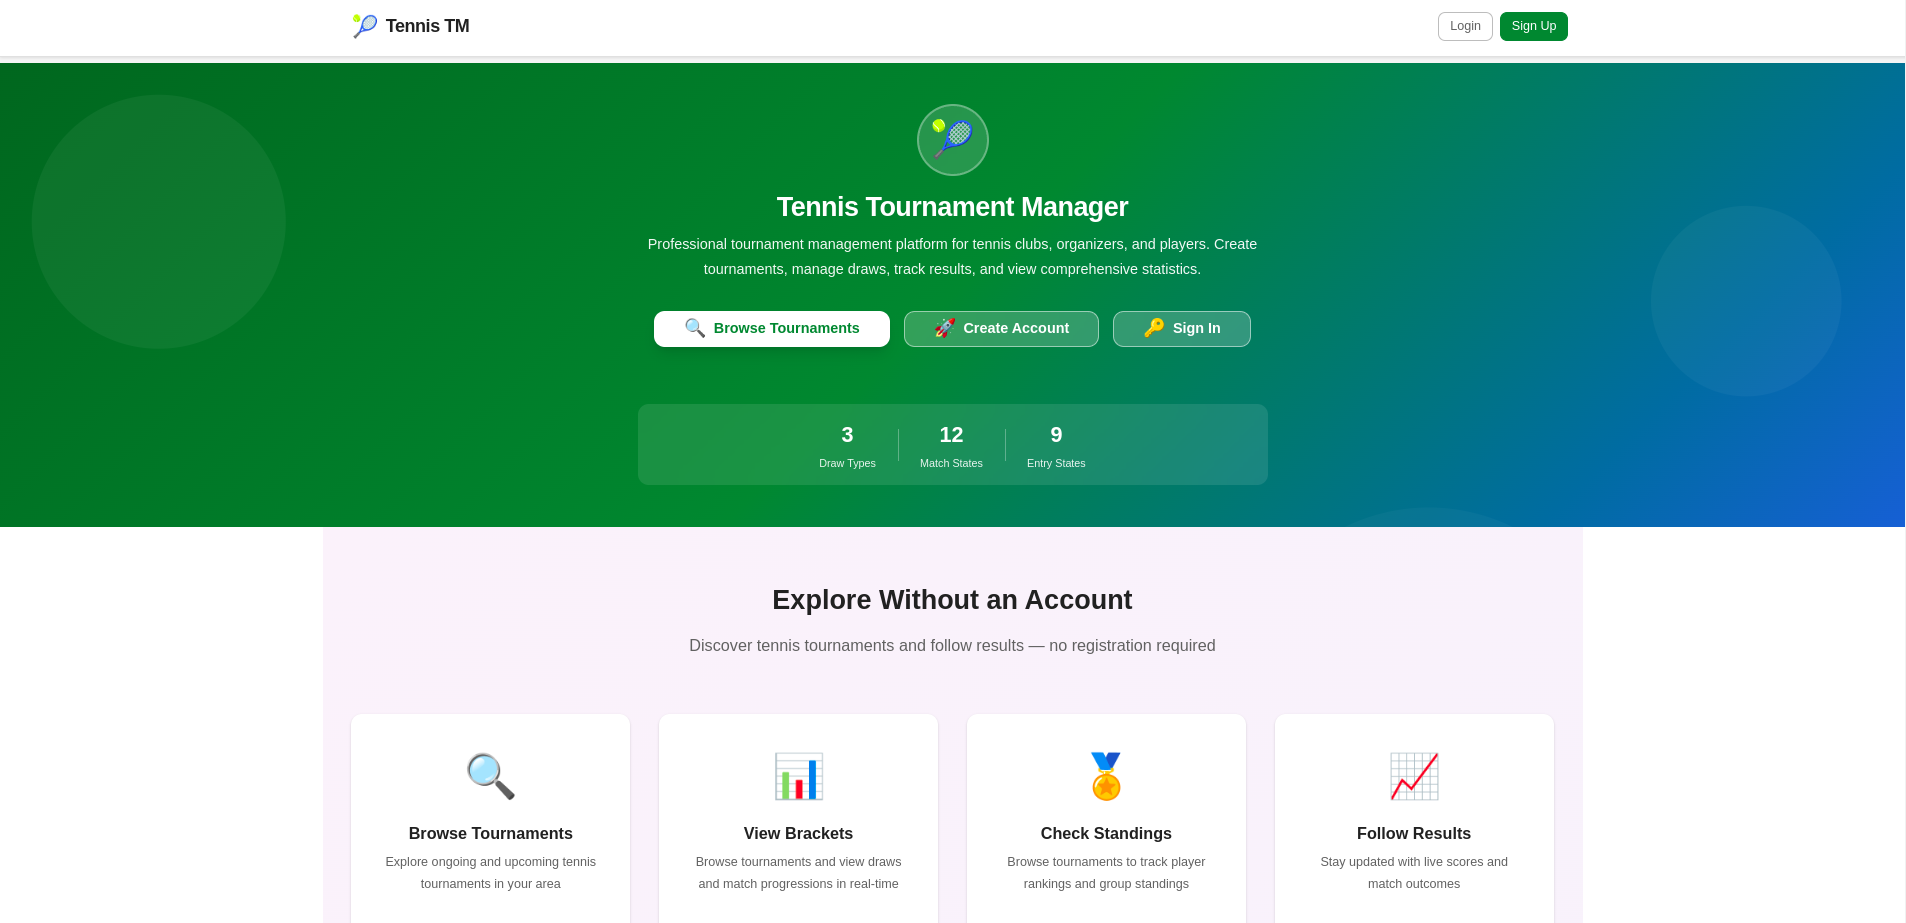
\includegraphics[width=\textwidth]{images/tennis-ui-after}
    %\caption*{\textit{Después}: diseño homogeneizado tras las correcciones de estilo.}
  \end{minipage}
  \caption{Interfaz de \ac{TENNIS} antes (izquierda) y después (derecha) de la fase de corrección de estilos.}
  \label{fig:tennis-ui-before-after}
\end{figure}

\section{Fase de Revisión} \label{sec:dev-review}
\subsection{P1--P3: revisión por módulos}
En \ac{HANGMAN}, la \ac{IA} Revisora no se limitó a señalar la incidencia de \textit{WordDictionary}: generó autónomamente el fichero \texttt{animals.json} y reescribió el constructor de la clase para cargarlo mediante importación estática\footnote{\href{https://github.com/alu0101549491/TFG-Fabian-Gonzalez-Lence/blob/main/projects/1-TheHangmanGame/src/models/word-dictionary.ts\#L30-L34}{\texttt{word-dictionary.ts} — versión final con vocabulario externalizado}}, cerrando la incidencia. 
Fue el primer indicio de que la IA Revisora podía absorber correcciones de implementación, capacidad que el enfoque basado en agentes explotaría de forma sistemática a partir de \ac{CARTO}. El resto de módulos recibieron veredicto aprobado en su primera revisión\footnote{\href{https://github.com/alu0101549491/TFG-Fabian-Gonzalez-Lence/tree/main/resources/prompts/1-TheHangmanGame/4-RevisionPorModulo}{\textit{Prompts} de revisión de \texttt{HANGMAN}}}.

En \ac{PLAYER}, las indicaciones de la revisión\footnote{\href{https://github.com/alu0101549491/TFG-Fabian-Gonzalez-Lence/tree/main/resources/prompts/2-MusicWebPlayer/4-RevisionPorModulo}{\textit{Prompts} de revisión de \texttt{PLAYER}}} se aplicaron de forma manual: la \ac{IA} Revisora señalaba el problema y se trasladaba a la \ac{IA} Desarrolladora para corregirlo, sin generar el código de corrección de forma autónoma.

En \ac{BALATRO}, la revisión requirió tres pasadas\footnote{\href{https://github.com/alu0101549491/TFG-Fabian-Gonzalez-Lence/tree/main/resources/prompts/3-MiniBalatro/4-RevisionPorGrupodeModulos}{\textit{Prompts} de revisión de \texttt{BALATRO}}} frente a la única pasada de los proyectos anteriores. La primera introdujo dos cambios arquitectónicos: la incorporación de identificadores únicos a las cartas \textit{Tarot} y la externalización de los datos de balanceo a cuatro ficheros JSON (\texttt{hand-values.json}, \texttt{jokers.json}, \texttt{planets.json} y \texttt{tarots.json}), con la reescritura de la clase \textit{BalancingConfig} para cargarlos de forma asíncrona. La segunda consolidó la lógica de la clase \textit{HandEvaluator} ---que duplicaba 160 líneas de sentencias \textit{switch-case} entre los métodos \textit{evaluateHand()} y \textit{getHandType()}--- y unificó el método \textit{canActivate()} de las subclases de \textit{Joker} en la clase base. La tercera resolvió errores de integración entre los componentes React y el resto del proyecto\footnote{\href{https://github.com/alu0101549491/TFG-Fabian-Gonzalez-Lence/blob/main/projects/3-MiniBalatro/docs/CODE_REVIEW_SUMMARY.md}{Resumen de revisión de código de \texttt{BALATRO}}}.

\subsection{P4--P5: metodología de tres etapas}

En \ac{CARTO}, la revisión\footnote{\href{https://github.com/alu0101549491/TFG-Fabian-Gonzalez-Lence/tree/main/resources/prompts/4-CartographicProjectManager/4-RevisionDelCodigo}{\textit{Prompts} de revisión de \texttt{CARTO}}} siguió la metodología de tres etapas descrita en la Sección~\ref{sec:approach-change}: exploración y generación de lista de tareas sobre 41 grupos, revisión con producción de un informe\footnote{\href{https://github.com/alu0101549491/TFG-Fabian-Gonzalez-Lence/blob/main/projects/4-CartographicProjectManager/docs/review/reports/CODE_REVIEW_REPORT.md}{Informe de revisión de código de \texttt{CARTO}}} con 5 incidencias críticas, 30 altas, 111 medias y 79 bajas, y aplicación de correcciones prudentes. Las más relevantes fueron: enumeraciones de dominio que codificaban nombres de pantalla y colores propios de la capa de presentación, vulnerando la regla de dependencias de \textit{Clean Architecture}; secretos JWT\footnote{\href{https://es.wikipedia.org/wiki/JSON_Web_Token}{JSON Web Token}} sin valores de entorno obligatorios y con \textit{fallback} a cadenas vacías; \textit{tokens} de autenticación persistidos en \texttt{localStorage}; y operaciones \textit{WebSocket} ejecutables sin verificar autorización.

En \ac{TENNIS}, la misma metodología\footnote{\href{https://github.com/alu0101549491/TFG-Fabian-Gonzalez-Lence/tree/main/resources/prompts/5-TennisTournamentManager/4-RevisionDelCodigo}{\textit{Prompts} de revisión de \texttt{TENNIS}}} organizó la base de código en doce grupos y produjo un informe\footnote{\href{https://github.com/alu0101549491/TFG-Fabian-Gonzalez-Lence/blob/main/projects/5-TennisTournamentManager/docs/review_reports/TENNIS_review_report.md}{Informe de revisión de código de \texttt{TENNIS}}} con 60 incidencias. Las más graves fueron: el \textit{middleware} de administración verificaba el rol  ``\texttt{ADMIN}''  mientras la enumeración real definía \texttt{SYSTEM\_ADMIN} y \texttt{TOURNAMENT\_ADMIN}, bloqueando \textit{endpoints} protegidos; seis ramas de confirmación de resultados devolvían éxito sin persistir el cambio de estado ni notificar a los participantes; y cinco servicios referenciados por el contenedor de inyección de Angular sin proveedor registrado. Tras las correcciones\footnote{\href{https://github.com/alu0101549491/TFG-Fabian-Gonzalez-Lence/blob/main/projects/5-TennisTournamentManager/docs/review_reports/TENNIS_fix_report.md}{Informe de correcciones de \texttt{TENNIS}}}, 58 de las 60 incidencias fueron resueltas, siendo las dos restantes materia de la fase de pruebas.

\section{Fase de Pruebas} \label{sec:dev-testing}

\subsection{P1--P3: Pruebas unitarias con Jest}

En \ac{HANGMAN}, Qwen AI generó nueve conjuntos de pruebas unitarias\footnote{\href{https://github.com/alu0101549491/TFG-Fabian-Gonzalez-Lence/tree/main/resources/prompts/1-TheHangmanGame/5-TestingPorModulo}{\textit{Prompts} de \textit{testing} de \texttt{HANGMAN}}} distribuidas en las tres capas \ac{MVC}, de las cuales siete pasaron sin correcciones. Las dos excepciones compartían raíz: dependencia del entorno de Canvas bajo JSDOM. El fichero \texttt{hangman-renderer.test.ts} carecía de un \textit{mock} del contexto 2D\footnote{\href{https://github.com/alu0101549491/TFG-Fabian-Gonzalez-Lence/blob/main/projects/1-TheHangmanGame/tests/views/hangman-renderer.test.ts\#L28-L45}{\texttt{hangman-renderer.test.ts}, líneas 28--45}} y el fichero \texttt{game-view.test.ts} invocaba al método \textit{initialize()} antes de limpiar los contadores de \textit{mock}\footnote{\href{https://github.com/alu0101549491/TFG-Fabian-Gonzalez-Lence/blob/main/projects/1-TheHangmanGame/tests/views/game-view.test.ts\#L56-L67}{\texttt{game-view.test.ts}, líneas 56--67}}. Ambas se resolvieron con una cobertura final del 82\%.

En \ac{PLAYER}, veintiún conjuntos de pruebas\footnote{\href{https://github.com/alu0101549491/TFG-Fabian-Gonzalez-Lence/tree/main/resources/prompts/2-MusicWebPlayer/5-TestingPorModulo}{\textit{Prompts} de \textit{testing} de \texttt{PLAYER}}} cubrieron componentes, \textit{hooks}, tipos y utilidades; diecinueve pasaron correctamente. En \texttt{usePlaylist.test.ts}, la lógica de navegación con \textit{RepeatMode.ALL} fallaba al encadenar llamadas consecutivas al método \textit{next()} que cruzaban el límite de la lista\footnote{\href{https://github.com/alu0101549491/TFG-Fabian-Gonzalez-Lence/blob/main/projects/2-MusicWebPlayer/tests/hooks/usePlaylist.test.ts\#L248-L264}{\texttt{usePlaylist.test.ts}, líneas 248--264}}; en el fichero \texttt{error-handler.test.ts}, en un principio la prueba no distinguía correctamente entre \textit{MediaError} y errores genéricos de red\footnote{\href{https://github.com/alu0101549491/TFG-Fabian-Gonzalez-Lence/blob/main/projects/2-MusicWebPlayer/tests/utils/error-handler.test.ts\#L88-L100}{\texttt{error-handler.test.ts}, líneas 88--100}}. La cobertura final alcanzó el 80\%.

En \ac{BALATRO}, siete \textit{prompts} por grupos\footnote{\href{https://github.com/alu0101549491/TFG-Fabian-Gonzalez-Lence/tree/main/resources/prompts/3-MiniBalatro/5-TestingPorGrupodeModulos}{\textit{Prompts} de \textit{testing} de \texttt{BALATRO}}} produjeron quince ficheros en cuatro categorías ---modelos, servicios, controladores y utilidades--- más el fichero de integración \texttt{game-flow.test.ts}, el primero del experimento en ejercitar la comunicación entre capas. Los conjuntos del servicio de persistencia requirieron ajustes porque los \textit{mocks} no reproducían correctamente la deserialización ante estados incompletos; el test de integración necesitó una segunda iteración para modelar la secuencia de transiciones del ciclo de partida. Los componentes React se excluyeron del cómputo de cobertura por diseño. La cobertura alcanzó un 70\%.

\subsection{P4--P5: Playwright \textit{end-to-end}}

En \ac{CARTO}, el agente recibió primero un \textit{prompt} de definición de escenarios\footnote{\href{https://github.com/alu0101549491/TFG-Fabian-Gonzalez-Lence/blob/main/resources/prompts/4-CartographicProjectManager/5-TestingDeLaAplicacion/test-scenarios.prompt.md}{\textit{Prompt} de escenarios de \texttt{CARTO}}} ---a partir de los diagramas de casos de uso y las rutas implementadas--- y en una segunda interacción un \textit{prompt} de implementación\footnote{\href{https://github.com/alu0101549491/TFG-Fabian-Gonzalez-Lence/blob/main/resources/prompts/4-CartographicProjectManager/5-TestingDeLaAplicacion/test-implementations.prompt.md}{\textit{Prompt} de implementación de \texttt{CARTO}}} que materializó esos escenarios en código con Playwright. Se generaron aproximadamente 400 pruebas en veinte conjuntos de tres niveles de criticidad; la batería crítica cubre autenticación, CRUD\footnote{\href{https://es.wikipedia.org/wiki/CRUD}{CRUD}} de proyectos y tareas, mensajería, gestión de ficheros y notificaciones en tiempo real. Los conjuntos requirieron correcciones de configuración de entorno para que el agente pudiera sembrar y limpiar datos de prueba vía \ac{API}.

En \ac{TENNIS}, el mismo flujo de dos \textit{prompts}\footnote{\href{https://github.com/alu0101549491/TFG-Fabian-Gonzalez-Lence/blob/main/resources/prompts/5-TennisTournamentManager/5-TestingDeLaAplicacion/test-scenarios.prompt.md}{\textit{Prompt} de escenarios de \texttt{TENNIS}}} \footnote{\href{https://github.com/alu0101549491/TFG-Fabian-Gonzalez-Lence/blob/main/resources/prompts/5-TennisTournamentManager/5-TestingDeLaAplicacion/test-implementations.prompt.md}{\textit{Prompt} de implementación de \texttt{TENNIS}}} generó 23 ficheros de pruebas en cuatro niveles de criticidad, cubriendo autenticación, gestión de torneos, cuadros, orden de juego, clasificaciones, anuncios y notificaciones. El conjunto se amplió en dos pasadas adicionales\footnote{\href{https://github.com/alu0101549491/TFG-Fabian-Gonzalez-Lence/tree/main/resources/prompts/5-TennisTournamentManager/5-TestingDeLaAplicacion}{\textit{Prompts} de ampliación de pruebas}} derivadas de la sesión de retroalimentación (Sección~\ref{sec:dev-client-feedback}).

\section{Retroalimentación de los clientes} \label{sec:dev-client-feedback}

El cliente de \ac{CARTO} valoró positivamente la aplicación ---estimando una cobertura del 95\% de sus expectativas--- y solicitó cuatro mejoras puntuales\footnote{\href{https://github.com/alu0101549491/TFG-Fabian-Gonzalez-Lence/tree/main/resources/prompts/4-CartographicProjectManager/6-PeticionesDelCliente}{\textit{Prompts} de peticiones del cliente de \texttt{CARTO}}}: la eliminación de la validación por expresión regular del código de proyecto en favor de un formato libre; la actualización del catálogo de tipos de proyecto a doce categorías del dominio cartográfico, con la correspondiente migración de esquema; la inclusión de una tarjeta en el panel de control con indicador de tareas pendientes asignadas al usuario autenticado; y la corrección de la integración con Dropbox, que no reflejaba los ficheros subidos directamente ni eliminaba el directorio del proyecto al borrarlo en la aplicación. El agente implementó cada mejora en sesiones de \textit{prompt} independientes sin modificar la arquitectura funcional existente.

El cliente de \ac{TENNIS} realizó una evaluación formal de la aplicación\footnote{\href{https://github.com/alu0101549491/TFG-Fabian-Gonzalez-Lence/blob/main/resources/prompts/5-TennisTournamentManager/6-FeedbackDeLaAplicacion/client-feedback.prompt.md}{\textit{Prompt} de retroalimentación del cliente de \texttt{TENNIS}}} y señaló deficiencias en la navegación, la visualización de encuentros y la distinción entre estados de partido. El agente elaboró un plan de implementación\footnote{\href{https://github.com/alu0101549491/TFG-Fabian-Gonzalez-Lence/blob/main/projects/5-TennisTournamentManager/docs/FEEDBACK-IMPLEMENTATION-PLAN.md}{Plan de implementación de retroalimentación de \texttt{TENNIS}}} y ejecutó los cambios en sesiones sucesivas\footnote{\href{https://github.com/alu0101549491/TFG-Fabian-Gonzalez-Lence/tree/main/resources/prompts/5-TennisTournamentManager/6-FeedbackDeLaAplicacion}{\textit{Prompts} de retroalimentación de \texttt{TENNIS}}}: corrigió veinticinco botones de retroceso distribuidos por toda la aplicación, estandarizó el comportamiento de navegación entre formularios e implementó el sistema de \textit{phase-linking}\footnote{\href{https://github.com/alu0101549491/TFG-Fabian-Gonzalez-Lence/blob/main/resources/prompts/5-TennisTournamentManager/6-FeedbackDeLaAplicacion/phase-linking.prompt.md}{\textit{Prompt} de \textit{phase-linking}}} ---vinculación de la fase clasificatoria con el cuadro principal--- que automatizaba el traspaso de los jugadores de una fase a otra, ya sea del mismo torneo o entre varios.
